% ------------------------------------------------------------
% LaTeX Template für die DHBW zum Schnellstart!
% Original: https://github.wdf.sap.corp/vtgermany/LaTeX-Template-DHBW
% ------------------------------------------------------------
% ---- Präambel mit Angaben zum Dokument
\documentclass[
	fontsize=12pt,           % Leitlinien sprechen von Schriftgröße 12.
	paper=A4,
	twoside=false,
	listof=totoc,            % Tabellen- und Abbildungsverzeichnis ins Inhaltsverzeichnis
	bibliography=totoc,      % Literaturverzeichnis ins Inhaltsverzeichnis aufnehmen
	titlepage,               % Titlepage-Umgebung anstatt \maketitle
	headsepline,             % horizontale Linie unter Kolumnentitel
	abstract,              % Überschrift einschalten, Abstract muss in {abstract}-Umgebung stehen
]{scrreprt}                  % Verwendung von KOMA-Report
\usepackage[utf8]{inputenc}  % UTF8 Encoding einschalten
\usepackage[english]{babel}  % Neue deutsche Rechtschreibung
\usepackage[T1]{fontenc}     % Ausgabe von westeuropäischen Zeichen (auch Umlaute)
\usepackage{microtype}       % Trennung von Wörtern wird besser umgesetzt
\usepackage{lmodern}         % Nicht-gerasterte Schriftarten (bei MikTeX erforderlich)
\usepackage{graphicx}        % Einbinden von Grafiken erlauben
\usepackage{wrapfig}         % Grafiken fließend im Text
\usepackage{setspace}        % Zeilenabstand \singlespacing, \onehalfspaceing, \doublespacing
\usepackage[
	%showframe,                % Ränder anzeigen lassen
	left=2.7cm, right=2.5cm,
	top=2.5cm,  bottom=2.5cm,
	includeheadfoot
]{geometry}                      % Seitenlayout einstellen
\usepackage{scrlayer-scrpage}    % Gestaltung von Fuß- und Kopfzeilen
\usepackage{acronym}             % Abkürzungen, Abkürzungsverzeichnis
\usepackage{titletoc}            % Anpassungen am Inhaltsverzeichnis
\contentsmargin{0.75cm}          % Abstand im Inhaltsverzeichnis zw. Punkt und Seitenzahl
\usepackage[                     % Klickbare Links (enth. auch "nameref", "url" Package)
  hidelinks,                     % Blende die "URL Boxen" aus.
  breaklinks=true                % Breche zu lange URLs am Zeilenende um
]{hyperref}
\usepackage[hypcap=true]{caption}% Anker Anpassung für Referenzen
\urlstyle{same}                  % Aktuelle Schrift auch für URLs
% Anpassung von autoref für Gleichungen (ergänzt runde Klammern) und Algorithm.
% Anstatt "Listing" kann auch z.B. "Code-Ausschnitt" verwendet werden. Dies sollte
% jedoch synchron gehalten werden mit \lstlistingname (siehe weiter unten).
%\addto\extrasngerman{%
%	\def\equationautorefname~#1\null{Gleichung~(#1)\null}
%	\def\lstnumberautorefname{Zeile}
%	\def\lstlistingautorefname{Listing}
%	\def\algorithmautorefname{Algorithmus}
%	% Damit einheitlich "Abschnitt 1.2[.3]" verwendet wird und nicht "Unterabschnitt 1.2.3"
%	% \def\subsectionautorefname{Abschnitt}
%}

% ---- Abstand verkleinern von der Überschrift
\renewcommand*{\chapterheadstartvskip}{\vspace*{.5\baselineskip}}

% Hierdurch werden Schusterjungen und Hurenkinder vermieden, d.h. einzelne Wörter
% auf der nächsten Seite oder in einer einzigen Zeile.
% LaTeX kann diese dennoch erzeugen, falls das Layout ansonsten nicht umsetzbar ist.
% Diese Werte sind aber gute Startwerte.
\widowpenalty10000
\clubpenalty10000

% ---- Für das Quellenverzeichnis
\usepackage[
	backend = biber,                % Verweis auf biber
	language = auto,
	style = numeric,                % Nummerierung der Quellen mit Zahlen
	sorting = none,                 % none = Sortierung nach der Erscheinung im Dokument
	sortcites = true,               % Sortiert die Quellen innerhalb eines cite-Befehls
	block = space,                  % Extra Leerzeichen zwischen Blocks
	hyperref = true,                % Links sind klickbar auch in der Quelle
	%backref = true,                % Referenz, auf den Text an die zitierte Stelle
	bibencoding = auto,
	giveninits = true,              % Vornamen werden abgekürzt
	doi=false,                      % DOI nicht anzeigen
	isbn=false,                     % ISBN nicht anzeigen
    alldates=short                  % Datum immer als DD.MM.YYYY anzeigen
]{biblatex}
\addbibresource{Inhalt/literatur.bib}
\setcounter{biburlnumpenalty}{3000}     % Umbruchgrenze für Zahlen
\setcounter{biburlucpenalty}{6000}      % Umbruchgrenze für Großbuchstaben
\setcounter{biburllcpenalty}{9000}      % Umbruchgrenze für Kleinbuchstaben
\DeclareNameAlias{default}{family-given}  % Nachname vor dem Vornamen
\AtBeginBibliography{\renewcommand{\multinamedelim}{\addslash\space
}\renewcommand{\finalnamedelim}{\multinamedelim}}  % Schrägstrich zwischen den Autorennamen
%\DefineBibliographyStrings{german}{
%  urlseen = {Einsichtnahme:},                      % Ändern des Titels von "besucht am"
%}
\usepackage[babel]{csquotes}


% ---- Für Mathevorlage
\usepackage{amsmath}    % Erweiterung vom Mathe-Satz
\usepackage{amssymb}    % Lädt amsfonts und weitere Symbole
\usepackage{MnSymbol}   % Für Symbole, die in amssymb nicht enthalten sind.


% ---- Für Quellcodevorlage
\usepackage{scrhack}                    % Hack zur Verw. von listings in KOMA-Script
\usepackage{listings}                   % Darstellung von Quellcode
\usepackage{xcolor}                     % Einfache Verwendung von Farben
% -- Eigene Farben für den Quellcode
\definecolor{JavaLila}{rgb}{0.4,0.1,0.4}
\definecolor{JavaGruen}{rgb}{0.3,0.5,0.4}
\definecolor{JavaBlau}{rgb}{0.0,0.0,1.0}
\definecolor{ABAPKeywordsBlue}{HTML}{6000ff}
\definecolor{ABAPCommentGrey}{HTML}{808080}
\definecolor{ABAPStringGreen}{HTML}{4da619}
\definecolor{PyKeywordsBlue}{HTML}{0000AC}
\definecolor{PyCommentGrey}{HTML}{808080}
\definecolor{PyStringGreen}{HTML}{008080}
% -- Farben für ABAP CDS
\definecolor{CDSString}{HTML}{FF8C00}
\definecolor{CDSKeywords}{HTML}{6000ff}
\definecolor{CDSAnnotation}{HTML}{00BFFF}
\definecolor{CDSComment}{HTML}{808080}
\definecolor{CDSFunc}{HTML}{FF0000}

% -- Default Listing-Styles

\lstset{
	% Das Paket "listings" kann kein UTF-8. Deswegen werden hier 
	% die häufigsten Zeichen definiert (ä,ö,ü,...)
	literate=%
		{á}{{\'a}}1 {é}{{\'e}}1 {í}{{\'i}}1 {ó}{{\'o}}1 {ú}{{\'u}}1
		{Á}{{\'A}}1 {É}{{\'E}}1 {Í}{{\'I}}1 {Ó}{{\'O}}1 {Ú}{{\'U}}1
		{à}{{\`a}}1 {è}{{\`e}}1 {ì}{{\`i}}1 {ò}{{\`o}}1 {ù}{{\`u}}1
		{À}{{\`A}}1 {È}{{\'E}}1 {Ì}{{\`I}}1 {Ò}{{\`O}}1 {Ù}{{\`U}}1
		{ä}{{\"a}}1 {ë}{{\"e}}1 {ï}{{\"i}}1 {ö}{{\"o}}1 {ü}{{\"u}}1
		{Ä}{{\"A}}1 {Ë}{{\"E}}1 {Ï}{{\"I}}1 {Ö}{{\"O}}1 {Ü}{{\"U}}1
		{â}{{\^a}}1 {ê}{{\^e}}1 {î}{{\^i}}1 {ô}{{\^o}}1 {û}{{\^u}}1
		{Â}{{\^A}}1 {Ê}{{\^E}}1 {Î}{{\^I}}1 {Ô}{{\^O}}1 {Û}{{\^U}}1
		{œ}{{\oe}}1 {Œ}{{\OE}}1 {æ}{{\ae}}1 {Æ}{{\AE}}1 {ß}{{\ss}}1
		{ű}{{\H{u}}}1 {Ű}{{\H{U}}}1 {ő}{{\H{o}}}1 {Ő}{{\H{O}}}1
		{ç}{{\c c}}1 {Ç}{{\c C}}1 {ø}{{\o}}1 {å}{{\r a}}1 {Å}{{\r A}}1
		{€}{{\euro}}1 {£}{{\pounds}}1 {«}{{\guillemotleft}}1
		{»}{{\guillemotright}}1 {ñ}{{\~n}}1 {Ñ}{{\~N}}1 {¿}{{?`}}1,
	breaklines=true,        % Breche lange Zeilen um 
	breakatwhitespace=true, % Wenn möglich, bei Leerzeichen umbrechen
	% Symbol für Zeilenumbruch einfügen
	prebreak=\raisebox{0ex}[0ex][0ex]{\ensuremath{\rhookswarrow}},
	postbreak=\raisebox{0ex}[0ex][0ex]{\ensuremath{\rcurvearrowse\space}},
	tabsize=4,                                 % Setze die Breite eines Tabs
	basicstyle=\ttfamily\small,                % Grundsätzlicher Schriftstyle
	columns=fixed,                             % Besseres Schriftbild
	numbers=left,                              % Nummerierung der Zeilen
	%frame=single,                             % Umrandung des Codes
	showstringspaces=false,                    % Keine Leerzeichen hervorheben
	keywordstyle=\color{blue},
	ndkeywordstyle=\bfseries\color{darkgray},
	identifierstyle=\color{black},
	commentstyle=\itshape\color{JavaGruen},   % Kommentare in eigener Farbe
	stringstyle=\color{JavaBlau},             % Strings in eigener Farbe,
	captionpos=b,                             % Bild*unter*schrift
	xleftmargin=5.0ex
}

% ---- Eigener JAVA-Style für den Quellcode
\renewcommand{\ttdefault}{pcr}               % Schriftart, welche auch fett beinhaltet
\lstdefinestyle{EigenerJavaStyle}{
	language=Java,                             % Syntax Highlighting für Java
	%frame=single,                             % Umrandung des Codes
	keywordstyle=\bfseries\color{JavaLila},    % Keywords in eigener Farbe und fett
	commentstyle=\itshape\color{JavaGruen},    % Kommentare in eigener Farbe und italic
	stringstyle=\color{JavaBlau}               % Strings in eigener Farbe
}

% ---- Eigener ABAP-Style für den Quellcode
\renewcommand{\ttdefault}{pcr}
\lstdefinestyle{EigenerABAPStyle}{
	language=[R/3 6.10]ABAP,
	morestring=[b]\|,                          % Für Pipe-Strings
	morestring=[b]\`,                          % für Backtick-Strings
	keywordstyle=\bfseries\color{ABAPKeywordsBlue},
	commentstyle=\itshape\color{ABAPCommentGrey},
	stringstyle=\color{ABAPStringGreen},
	tabsize=2,
	morekeywords={
		types,
		@data,
		as,
		lower,
		start,
		selection,
		order,
		by,
		inner,
		join,
		key,
		end,
		cast
	}
}

% ---- Eigener Python-Style für den Quellcode
\renewcommand{\ttdefault}{pcr}
\lstdefinestyle{EigenerPythonStyle}{
	language=Python,
	columns=flexible,
	keywordstyle=\bfseries\color{PyKeywordsBlue},
	commentstyle=\itshape\color{PyCommentGrey},
	stringstyle=\color{PyStringGreen}
}

%----- ABAP-CDS-View language
\lstdefinelanguage{ABAPCDS}{
	sensitive=false,
	%Keywords
	morekeywords={define,
		view,
		as,
		select,
		from,
		inner,
		join,
		on,
		key,
		case,
		when,
		then,
		else,
		end,
		true,
		false,
		cast,
		where,
		and,
		distinct,
		group,
		by,
		having,
		min,
		sum,
		max,
		count,
		avg
	},
	%Methoden
	morekeywords=[2]{
		div,
		currency\_conversion,
		dats\_days\_between,
		concat\_with\_space,
		dats\_add_days,
		dats\_is\_valid,
		dats\_add\_months,
		unit\_conversion,
		division,
		mod,
		abs,
		floor,
		ceil,
		round,
		concat,
		replace,
		substring,
		left,
		right,
		length
	},
	morecomment=[s][\color{CDSAnnotation}]{@}{:},
	morecomment=[l][\itshape\color{CDSComment}]{//},
	morecomment=[s][\itshape\color{CDSComment}]{/*}{*/},
	morestring=[b][\color{CDSString}]',
	keywordstyle=\bfseries\color{CDSKeywords},
	keywordstyle=[2]\color{CDSFunc}
}

  % Weitere Details sind ausgelagert

\usepackage{algorithm}                  % Für Algorithmen-Umgebung (ähnlich wie lstlistings Umgebung)
\usepackage{algpseudocode}              % Für Pseudocode. Füge "[noend]" hinzu, wenn du kein "endif",
                                        % etc. haben willst.

\makeatletter                           % Sorgt dafür, dass man @ in Namen verwenden kann.
                                        % Ansonsten gibt es in der nächsten Zeile einen Compilefehler.
%\renewcommand{\ALG@name}{Algorithmus}   % Umbenennen von "Algorithm" im Header der Listings.
\makeatother                            % Zeichen wieder zurücksetzen
\renewcommand{\lstlistingname}{Listing} % Erlaubt das Umbenennen von "Listing" in anderen Titel.

% ---- Tabellen
\usepackage{booktabs}  % Für schönere Tabellen. Enthält neue Befehle wie \midrule
\usepackage{multirow}  % Mehrzeilige Tabellen
\usepackage{siunitx}   % Für SI Einheiten und das Ausrichten Nachkommastellen
\sisetup{locale=DE, range-phrase={~bis~}, output-decimal-marker={,}} % Damit ein Komma und kein Punkt verwendet wird.
\usepackage{xfrac} % Für siunitx Option "fraction-function=\sfrac"

% ---- Für Definitionsboxen in der Einleitung
\usepackage{amsthm}                     % Liefert die Grundlagen für Theoreme
\usepackage[framemethod=tikz]{mdframed} % Boxen für die Umrandung
% ---- Definition für Highlight Boxen

% ---- Grundsätzliche Definition zum Style
%\newtheoremstyle{defi}
%  {\topsep}         % Abstand oben
%  {\topsep}         % Abstand unten
%  {\normalfont}     % Schrift des Bodys
%  {0pt}             % Einschub der ersten Zeile
%  {\bfseries}       % Darstellung von der Schrift in der Überschrift
%  {:}               % Trennzeichen zwischen Überschrift und Body
%  {.5em}            % Abstand nach dem Trennzeichen zum Body Text
%  {\thmname{#3}}    % Name in eckigen Klammern
%\theoremstyle{defi}

% ------ Definition zum Strich vor eines Texts
\newmdtheoremenv[
  hidealllines = true,       % Rahmen komplett ausblenden
  leftline = true,           % Linie links einschalten
  innertopmargin = 0pt,      % Abstand oben
  innerbottommargin = 4pt,   % Abstand unten
  innerrightmargin = 0pt,    % Abstand rechts
  linewidth = 3pt,           % Linienbreite
  linecolor = gray!40,       % Linienfarbe
]{defStrich}{Definition}     % Name der des formats "defStrich"

% ------ Definition zum Eck-Kasten um einen Text
\newmdtheoremenv[
  hidealllines = true,
  innertopmargin = 6pt,
  linecolor = gray!40,
  singleextra={              % Eck-Markierungen für die Definition
    \draw[line width=3pt,gray!50,line cap=rect] (O|-P) -- +(1cm,0pt);
    \draw[line width=3pt,gray!50,line cap=rect] (O|-P) -- +(0pt,-1cm);
    \draw[line width=3pt,gray!50,line cap=rect] (O-|P) -- +(-1cm,0pt);
    \draw[line width=3pt,gray!50,line cap=rect] (O-|P) -- +(0pt,1cm);
  }
]{defEckKasten}{Definition}  % Name der des formats "defEckKasten"  % Weitere Details sind ausgelagert

% ---- Für Todo Notes
\usepackage{todonotes}
\setlength {\marginparwidth }{2cm}      % Abstand für Todo Notizen

% ---- Zum Einbinden von PDF-Dokumenten
\usepackage{pdfpages}


% ---- Elektronische Version oder Gedruckte Version?
% ---- Unterschied: Die elektronische Version enthält keinen Platzhalter für die Unterschrift
\usepackage{ifthen}
\newboolean{e-Abgabe}
\setboolean{e-Abgabe}{false}    % false=gedruckte Fassung

% ---- Persönlichen Daten:
\newcommand{\titel}{Template \LaTeX\ Wiki von BAzubis für BAzubis}
\newcommand{\titelheader}{Titel welcher im Header auftaucht}
\newcommand{\arbeit}{Projektarbeit 1 (T3\_2000)}
\newcommand{\studiengang}{Informatik}
\newcommand{\studienjahr}{2015}
\newcommand{\autor}{Vorname Nachname}
\newcommand{\autorReverse}{Nachname, Vorname}
\newcommand{\verfassungsort}{Karlsruhe}
\newcommand{\matrikelnr}{0000000}
\newcommand{\kurs}{TINF15B1}
\newcommand{\bearbeitungsmonat}{Januar 2025}
\newcommand{\abgabe}{01. Februar 2025}
\newcommand{\bearbeitungszeitraum}{01.10.2024 - 31.01.2025}
\newcommand{\firmaName}{SAP SE}
\newcommand{\firmaStrasse}{Dietmar-Hopp-Allee 16}
\newcommand{\firmaPlz}{69190 Walldorf, Deutschland}
\newcommand{\betreuerFirma}{B-Vorname B-Nachname}
\newcommand{\betreuerDhbw}{DH-Vorname DH-Nachname}

% ---- Metainformation für das PDF Dokument
\hypersetup{
	pdftitle    = {\titel},
	pdfsubject  = {\arbeit},
	pdfauthor   = {\autor},
	%pdfkeywords = {Keywords angeben},
	pdfcreator  = {LaTeX},
	%pdfproducer = {in der Regel pdfTeX}
}

% ---- Definition der Kopf- und Fußzeilen
\clearpairofpagestyles                          % Löschen von LaTeX Standard
\automark[section]{chapter}                     % Füllen von section und chapter
\renewcommand*{\chaptermarkformat}{}            % Entfernt die Kapitelnummer
\renewcommand*{\sectionmarkformat}{}            % Entfernt die Sectionnummer
% Angaben [für "plain"]{für "scrheadings"}
\ihead[]{\titelheader}                          % Kopfzeile links
\chead[]{}                                      % Kopfzeile mitte
\ohead[]{\rightmark}                            % Kopfzeile rechts
\ifoot[]{}                                      % Fußzeile links
\cfoot*{\sffamily\pagemark}                     % Fußzeile mitte
\ofoot[]{}                                      % Fußzeile rechts
\KOMAoptions{
   headsepline = 0.2pt,                         % Liniendicke Kopfzeile
   footsepline = false                          % Liniendicke Fußzeile
}


% ---- Hilfreiches
\newcommand{\zB}{z.\,B. }   % "z.B." mit kleinem Leeraum dazwischen (ohne wäre nicht korrekt)
\newcommand{\dash}{d.\,h. }

\newcommand{\code}[1]{\texttt{#1}} % Ist einfacher zu schreiben als ständig \texttt und erlaubt
                                   % Änderungen im Nachhinein, wenn man z.B. Inline-Code anders stylen möchte.

% ---- Silbentrennung (falls LaTeX defaults falsch / nicht gewünscht sind)
\hyphenation{HANA}         % anstatt HA-NA
\hyphenation{Graph-Script} % anstatt GraphS-cript

% ---- Beginn des Dokuments
\begin{document}
\setlength{\parindent}{0pt}              % Keine Paragraphen Einrückung.
                                         % Dafür haben wir den Abstand zwischen den Paragraphen.
\setcounter{secnumdepth}{2}              % Nummerierungstiefe fürs Inhaltsverzeichnis
\setcounter{tocdepth}{1}                 % Tiefe des Inhaltsverzeichnisses. Ggf. so anpassen,
                                         % dass das Verzeichnis auf eine Seite passt.
\sffamily                                % Serifenlose Schrift verwenden.

% ---- Vorspann
% ------ Titelseite
\singlespacing
\thispagestyle{empty}
\begin{titlepage}
\enlargethispage{4cm}

\begin{figure}           % Logo vom Ausbildungsbetrieb und der DHBW
	% \vspace*{-5mm} % Sollte dein Titel zu lang werden, kannst du mit diesem "Hack" 
	%                  den Inhalt der Seite nach oben schieben.
	\begin{minipage}{0.49\textwidth}
		\flushleft
		%\includegraphics[height=2.5cm]{Bilder/Logos/Logo_SAP.pdf} 
	\end{minipage}
	\hfill
	\begin{minipage}{0.49\textwidth}
		\flushright
		%\includegraphics[height=2.5cm]{Bilder/Logos/Logo_DHBW.pdf} 
	\end{minipage}
\end{figure} 
\vspace*{0.1cm}

\begin{center}
	\huge{\textbf{\titel}}\\[1.5cm]
	\Large{\textbf{\arbeit}}\\[0.5cm]
	\normalsize{im Rahmen der Prüfung zum\\[1ex] \textbf{Master of Science (B.Sc.)}}\\[0.5cm]
	\Large{des Studienganges \studiengang}\\[1ex]
	\normalsize{an der Dualen Hochschule Baden-Württemberg Karlsruhe}\\[1cm]
	\normalsize{von}\\[1ex] \Large{\textbf{\autor}} \\[1cm]
	% Hinweis: Manche Dozenten möchten einen Hinweis auf den Sperrvermerk auf der Titelseite.
	% \large{{\color{red}- Sperrvermerk -}}\\[1cm]
\end{center}

\begin{center}
	\vfill
	\begin{tabular}{ll}
		Abgabedatum:                     & \abgabe \\[0.2cm]
		Bearbeitungszeitraum:            & \bearbeitungszeitraum \\[0.2cm]
		Matrikelnummer, Kurs:            & \matrikelnr , \kurs \\[0.2cm]
		Ausbildungsfirma:                & \firmaName \\
		                                 & \firmaStrasse \\
		                                 & \firmaPlz \\[0.2cm]
		Betreuer der Ausbildungsfirma:   & \betreuerFirma \\[0.2cm]
		Gutachter der Dualen Hochschule: & \betreuerDhbw \\[2cm]
	\end{tabular} 
\end{center}
\end{titlepage}
  % Titelseite
\newcounter{savepage}
\pagenumbering{Roman}                    % Römische Seitenzahlen
\onehalfspacing

% ------ Erklärung, Sperrvermerk, Abstact
\chapter*{Eidesstattliche Erklärung}
Ich versichere hiermit, dass ich meine \arbeit{} mit dem Thema:
\begin{quote}
	\textit{\titel}
\end{quote} 
gemäß § 5 der \enquote{Studien- und Prüfungsordnung DHBW Technik} vom 29. September 2017 selbstständig verfasst und keine anderen als die angegebenen Quellen und Hilfsmittel benutzt habe. Die Arbeit wurde bisher keiner anderen Prüfungsbehörde vorgelegt und auch nicht veröffentlicht.

\vspace{0.25cm}

Ich versichere zudem, dass die eingereichte elektronische Fassung mit der gedruckten Fassung übereinstimmt.

\vspace{1cm}

\verfassungsort, den \today \\[0.5cm]
\ifthenelse{\boolean{e-Abgabe}}
	{\underline{Gez. \autor}}
	{\makebox[6cm]{\hrulefill}}\\ 
\autorReverse

\renewcommand{\abstractname}{Abstract} % Veränderter Name für das Abstract
\begin{abstract}
\begin{addmargin}[1.5cm]{1.5cm}        % Erhöhte Ränder, für Abstract Look
\thispagestyle{plain}                  % Seitenzahl auf der Abstract Seite

\begin{center}
\small\textit{- English -}             % Angabe der Sprache für das Abstract
\end{center}

\vspace{0.25cm}

This is the starting point of the Abstract. For the final bachelor thesis, there must be an abstract included in your document. So, start now writing it in German and English. The abstract is a short summary with around 200 to 250 words.

\vspace{0.25cm}

Try to include in this abstract the main question of your work, the methods you used or the main results of your work.


\end{addmargin}
\end{abstract}
\renewcommand{\abstractname}{Abstract} % Veränderter Name für das Abstract
\begin{abstract}
\begin{addmargin}[1.5cm]{1.5cm}        % Erhöhte Ränder, für Abstract Look
\thispagestyle{plain}                  % Seitenzahl auf der Abstract Seite

\begin{center}
\small\textit{- Deutsch -}             % Angabe der Sprache für das Abstract
\end{center}

\vspace{0.25cm}

Dies ist der Beginn des Abstracts. Für die finale Bachelorarbeit musst du ein Abstract in deinem Dokument mit einbauen. So, schreibe es am besten jetzt in Deutsch und Englisch. Das Abstract ist eine kurze Zusammenfassung mit ca. 200 bis 250 Wörtern.

\vspace{0.25cm}

Versuche in das Abstract folgende Punkte aufzunehmen: Fragestellung der Arbeit, methodische Vorgehensweise oder die Hauptergebnisse deiner Arbeit.


\end{addmargin}
\end{abstract}

% ------ Inhaltsverzeichnis
\singlespacing
\tableofcontents

% ------ Verzeichnisse
\renewcommand*{\chapterpagestyle}{plain}
\pagestyle{plain}
\chapter*{Formelverzeichnis}
\addcontentsline{toc}{chapter}{Formelverzeichnis} % Hinzufügen zum Inhaltsverzeichnis 

% Definition des neuen Befehls für das Einfügen der Abkürzung der Einheit
\newcommand{\acrounit}[1]{
  \acroextra{\makebox[18mm][l]{\si[per-mode=fraction,fraction-function=\sfrac]{#1}}}
}
\begin{acronym}[dmin] % längstes Kürzel wird verw. für den Abstand zw. Kürzel u. Text

	% Alphabetisch selbst sortieren - nicht verwendete Formeln rausnehmen!
	% Allgemein: \acro{KÜRZEL}[ABKÜRZUNG]{\acrounit{SI-EINHEIT}BESCHREIBUNG}

	\acro{A}[\ensuremath{A}]{\acrounit{mm^2}Fläche}	
	\acro{D}[\ensuremath{D}]{\acrounit{mm}Werkstückdurchmesser}	
	\acro{dmin}[\ensuremath{d\textsubscript{min}}]{\acrounit{mm}kleinster Schaftdurchmesser}	
	\acro{L1}[\ensuremath{L\textsubscript{1}}]{\acrounit{mm}Länge des Werkstückes Nr. 1}	
	\acro{Fwinkel}[]{\acrounit{Grad}Freiwinkel}	
	\acro{Kwinkel}[]{\acrounit{Grad}Keilwinkel}

\end{acronym}

\chapter*{Abkürzungsverzeichnis}
\addcontentsline{toc}{chapter}{Abkürzungsverzeichnis} % Hinzufügen zum Inhaltsverzeichnis 

\begin{acronym}[WYSISWG] % längstes Kürzel wird verw. für den Abstand zw. Kürzel u. Text

	% Alphabetisch selbst sortieren - nicht verwendete Kürzel rausnehmen!
	\acro{AIR}{Adobe Integrated Runtime}
	\acro{AJAX}{Asynchronous Javascript and XML}
	\acro{ANSI}{American National Standards Institute}
	\acro{API}{Application Programming Interface}
	\acro{AR}{Augmented Reality}
	\acro{BAPI}{Business Application Programming Interface}
	\acro{BIOS}{Basic Input Output System}
	\acro{CDMA}{Code Division Multiple Access}
	\acro{HTTPS}{Hypertext Transfer Protocol Secure}
	\acro{ISBN}{Internationale Standardbuchnummer}
	\acrodefplural{ISBN}[ISBNs]{Internationale Standardbuchnummern}
	\acro{OLAP}{Online Analytical Processing}
	\acro{ORDBMS}{Object-Relational DataBase Management System}
	\acro{SDK}{Software Development Kit}
	\acro{SEO}{Search Engine Optimization}
	\acro{SSH}{Secure Shell}
	\acro{UEFI}{Unified Extensible Firmware Interface}
	\acro{USB}{Universal Serial Bus}
	\acro{VLAN}{Virtual Local Area Network}
	\acro{WYSISWG}{What You See Is What You Get}
	\acro{XSL}{Extensible Stylesheet Language}

\end{acronym}
\listoffigures                          % Erzeugen des Abbildungsverzeichnisses 
\listoftables                           % Erzeugen des Tabellenverzeichnisses
\renewcommand{\lstlistlistingname}{Quellcodeverzeichnis}
\lstlistoflistings                      % Erzeugen des Listenverzeichnisses
\setcounter{savepage}{\value{page}}


% ---- Inhalt der Arbeit
\cleardoublepage
\pagenumbering{arabic}                  % Arabische Seitenzahlen für den Hauptteil
\setlength{\parskip}{0.5\baselineskip}  % Abstand zwischen Absätzen
\rmfamily
\renewcommand*{\chapterpagestyle}{scrheadings}
\pagestyle{scrheadings}
\onehalfspacing

\chapter{Introduction}
% 1 Seite

	Feel introduced.
	
	\section{Motivation and Contribution}
	% 0.5 Seiten
	
		I am motivated.
	
	\section{Structure}
	% 0.5 Seiten
	
		This text is well-structured.
		
	\section{Hm}
	
		\blindtext

\chapter{Preliminaries}
% 0.5 Seiten

	\section{Linear Optimization}
	% 2 Seiten
	
	\section{Dantzig-Wolfe Decomposition}
	% 2 Seiten
	
	\section{Graph Theory}
	% 2 Seiten
	
	\section{Partition Refinement}
	% 2 Seiten
\chapter{Related Work}
% 2 Seiten (mal schauen)
\chapter{\acf{GCG}}
\label{chap:gcg}
% 1 Seite

	\begin{figure}[ht!]
		\centering
		\includesvg[scale=0.8]{Bilder/DrawIO/detection_overview}
		\caption{A simplified overview of the four major stages of solving a model with \acs{GCG}.}
		\label{fig:gcg:overview}
	\end{figure}

	In this chapter, we introduce \acf{GCG}, a decomposition solver which is based on the open-source MIP-Solver \ac{SCIP} \cite{gamrathExperimentsGenericDantzigWolfe2010}.
	Readers already experienced with GCG and its capabilities may still find some details and observations interesting.
	For a given problem, \acs{GCG} is able to perform an automatic Dantzig-Wolfe reformulation which is then solved using a branch-price-and-cut algorithm.
	Alternatively, \ac{GCG} support a special \textit{Benders-Mode} which reformulated the problem using Benders decomposition.
	
	In contrast to other open-source solvers like \acfreverse{BaPCod} \cite{sadykovBaPCodGenericBranchandprice2021} or commercial software such as \textit{SAS} \cite{SASDataAI} which rely solely on user-provided decompositions, \ac{GCG} is able to automatically detect different kinds of structures algorithmically, including but not limited to
	\begin{itemize}
		\item Single-Bordered structures
		\item Arrowhead structures using the third-party tool \acfreverse{hMETIS} \cite{karypisMultilevelHypergraphPartitioning1997}.
		\item Staircase structures
	\end{itemize}
	\todo{Entfernen und auf Kapitel vorher ref}
	
	The solving process in divided into multiple consecutive stages as shown in Figure \ref{fig:gcg:overview}. Each stage will be explained in more detail in the following section as needed.
	The detection in particular aims to make \ac{GCG} more accessible to a wider range of users which do not necessarily have the required theoretical background and practical experience to reformulate linear programs on their own.
	For more details about individual features and capabilities, we refer to the official documentation \cite{GCG}. \todo{Kurz die 4 Schritte aus Bild erwähnen und einen Satz}

	\section{Detection}
	% 2 Seiten, Detection Loop etc.
	
		\begin{figure}[ht!]
			\centering
			\includesvg[scale=0.7]{Bilder/DrawIO/detection_loop}
			\caption{A simplified overview of the detection process and its detection loop.}
			\label{fig:gcg:detectionloop}
		\end{figure}
	
		As mentioned in the introduction to this chapter, one integral part and distinguishing feature of \ac{GCG} is its detection framework.
		A simplified overview of the detection currently \footnote{\ac{GCG} version 3.5, as of 2025-07-18.} implemented in \ac{GCG} is shown in Figure \ref{fig:gcg:detectionloop}. For a more detailed visualization including additional information about how pre-solving is handled we refer to the official documentation \cite{GCG}.
		The framework consists of two major parts:
		
		\begin{enumerate}
			\item A \textbf{classification} step, in which a set of classifiers is partitioning the constraints (and variables) according to a certain property, producing one partition each.
			The goal of this step is to detect different underlying structures of the constraint matrix, which can be used during the detection loop to make more informed decisions about which constraints to assign to which block or master.
			Important classifiers for the remainder of this thesis are discussed in more detail in Section \ref{chap:gcg:classifiers}.
			\item The \textbf{detection loop}, which consists of a set of detectors which are responsible for assigning constraints either the master or to individual blocks.
			In round $n+1$ a detector receives a \textit{partial} decomposition, that is, a decomposition in which \textit{not all} constraints are assigned yet, from round $n$ as input and pushes a set of newly created (partial) decompositions to a queue.
			In case the user did not provide a partial decomposition as input in round $0$, the loop is initialized with a decomposition in which no constraint is assigned yet.
		\end{enumerate}
	
		\begin{figure}[ht!]
			\centering
			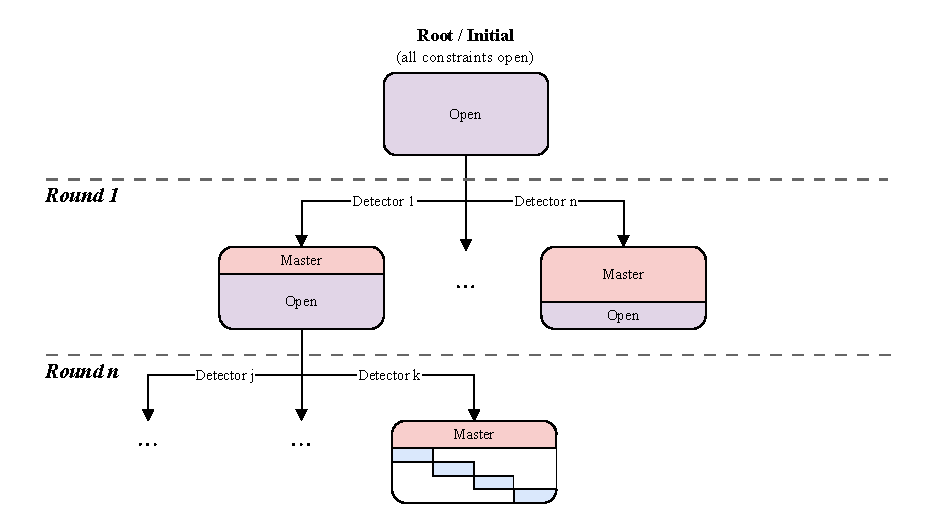
\includegraphics{Bilder/DrawIO/partialdec_tree_pdf}
			\caption{Visualization of the induced tree of propagated partial decompositions.}
			\label{fig:gcg:partialdettree}
		\end{figure}
		
		The concept of detecting structures in different rounds is visualized in Figure \ref{fig:gcg:partialdettree}.
		Starting from a root decomposition in which all constraints are still unassigned or \enquote{open}, different detectors produce a set of new partial decomposition.
		Depending on the configuration, a detector is not allowed to work on a certain partial decomposition or its decedents twice.
		A very simple but concrete example of how such a tree might look like in practice can be found in Section \ref{chap:gcg:example}.
		
		Furthermore, if no detector found any new decomposition in round $k$, or $k$ exceed the maximum number of rounds, the detection loop is stopped and all complete decomposition are collected, scored and exactly one is chosen for which the solving is started. \todo{Grammatik, Wortwahl}
		The scoring and selection stage is of particular interest in practice, because the tree in Figure \ref{fig:gcg:partialdettree} might grow beyond thousand of decompositions, of which the best in terms of solving time or a different metric must be selected.
		Because the scoring of decompositions is not of major interest for \textit{this} thesis, we refer to the official documentation for details \cite{GCG}.
	
	\clearpage
	
	\section{Classifiers}
	\label{chap:gcg:classifiers}
		% 1 Seite, Var Classifiers
		% 1 Seite, Cons Classifiers

		As mentioned in the introduction to this chapter, classifiers are responsible for detecting different underlying structures of the constraint matrix, which can be used during the detection loop to make more informed decisions about which constraints to assign to which block or master.
		Given a set of constraints $C = \{ c_1, c_2, \ldots, c_m \}$, classifiers can be seen as a \textit{injective} function $f: C \mapsto \mathbb{Z}$, i.e., a function that assigns each constraint to exactly one number or \textit{class}.
		Note that in \acs{GCG}, classifiers are allowed to only classify a subset $C' \subseteq C$, leaving $C \setminus C'$ unassigned to any class \footnote{When using \ac{GCG} as a library, this can be checked via. \lstinline|IndexPartition::isIndexClassified|.}.
		In the current version of \ac{GCG}, however, all classifiers always assign every constraint to some class.
		
		Furthermore, each classifier is identified with an unique \textit{name} and an integral priority, influencing the order in which the classifiers are being executed by the framework. 
		
		\subsection{Name Classifiers}
		\label{chap:gcg:classifiers:name}
		
			The names of constraints and variables are, if provided, a strong indicator to which constraints or variables are related to each other.
			The names usually consist of two parts:
			\begin{enumerate}
				\item The semantic group name, such as \enquote{capacity} or \enquote{link} for e.g. a Bin-Packing model. 
				\item A \textit{modifier}, which usually consists of numbers, capital letters or a combination of both. Typically, the modifier is separated from the semantic group name via.  non alpha-numeric characters such as \enquote{\_} or \enquote{\#}.
			\end{enumerate}
		
			Constraints in the same group typically share similar names, with the \textit{modifier} being the only differentiating factor. For example, in a Bin-Packing problem, capacity constraints such as \enquote{capacity\_1}, \enquote{capacity\_2}, $\ldots$ usually vary only in the index indicating the bin. This similarity can be quantified using metrics like the \textit{Levenshtein Distance}, which is the minimum number of single-character edits required to change one word into the other.
			
			\clearpage
			
			Because there is no standardized naming scheme for either variables or constraints, name classifiers usually operate under the assumption that the modeler provided \textit{reasonable} names, if any at all.
			A non-exhaustive collection of different naming schemes observed is provided in Appendix \todo{Appendix}.
			If the modelers provided no names of it's own, then the underlying solver usually chooses a default prefix such as \enquote{c} or \enquote{cons} for constraints, followed by an increasing number, resulting in constraint names \enquote{c0} - \enquote{c4999} for a model with 5000 constraints.
			
			Given a alphabet $\Sigma$, words $w, v \in \Sigma^*$, then the \textit{Levenshtein} distance between those two words can be computed as:
			%
			\begin{equation}
				\label{eq:gcg:levenshtein}
				\mathrm{lev}(w, v) = \begin{cases}
					|w| & \mathrm{if} \; v = \epsilon \\
					|v| & \mathrm{if} \; w = \epsilon \\
					\mathrm{lev}(\mathrm{prefix}(w), \mathrm{prefix}(v)) & \mathrm{if} \; \mathrm{head}(w) = \mathrm{head}(v) \\
					1 + \min \begin{cases}
						\mathrm{lev}(\mathrm{prefix}(w), v) \\
						\mathrm{lev}(w, \mathrm{prefix}(v)) \\
						\mathrm{lev}(\mathrm{prefix}(w), \mathrm{prefix}(v)) \\
					\end{cases} & \mathrm{otherwise}
				\end{cases}
			\end{equation}
			%
			Equation \ref{eq:gcg:levenshtein} can be computed in $O(|w| \cdot |v|)$ using a dynamic programming approach.
			Let $B = (\mathrm{lev}(\mathrm{name}(c_i), \mathrm{name}(c_j)))_{1 \leq i,j \leq m}$ the pair-wise Levenshtein Distance between constraint names, $k \in \mathbb{N}$ the \textit{connectivity} and $G = (V, E)$ with $V = \{ c_1, c_2, \ldots, c_m \}, E = \{ \{ u, v \} \mid u, v \in V, u \neq v, \mathrm{lev}(\mathrm{name}(u), \mathrm{name}(v)) \leq k \}$.
			Furthermore, let $reach(v)$ be the set of reachable vertices from vertex $v \in V$ which is defined as the fix-point of the following function for $s = v$:
			%
			\begin{equation*}
				{reachEventually}_t(T) = \{ u \in V \mid \exists v \in T: v \in E(u) \;  \} \cup \{ t \}
			\end{equation*}
			\todo{WIP}
			%
			Then two constraints $c_i, c_j \in V$ are in the same class iff $c_j \in reach(c_i)$.
			A small example of this concept is shown in Figure \ref{fig:gcg:levenshtein}.
			\todo{5000 cons limit}
			This idea can also be applied to variable names.
			
			\begin{figure}[ht!]
				\centering
				\includesvg[scale=0.8]{Bilder/DrawIO/levenshtein}
				\caption{The graph of pair-wise Levenshtein weights for three capacity constraints. For $k=1$, the edge between $capacity_3$ and $capacity_{12}$ vanishes, but because they is still a connecting path via. $capacity_1$, both constraints are assigned to the same class.}
				\label{fig:gcg:levenshtein}
			\end{figure}
			
			\FloatBarrier
		
		\subsection{Numeric Classifiers}
			
			\subsubsection{Nonzero}
			
				\begin{figure}[ht!]
					\centering
					\begin{equation*}
						A \; = \; \begin{pNiceMatrix}[first-row,first-col,last-col]
							& x_1 & x_2 & x_3 & x_4 & \; \textcolor{red}{class} \\
							{cons}_1 \; & 1 & 5 & -1 & -1 & \quad \textcolor{red}{4} \\
							{cons}_2 \; & 20 & 0 & 0 & 20 & \quad \textcolor{red}{2} \\
							{cons}_3 \;& 20 & 10 & 10 & 0 & \quad \textcolor{red}{3} \\
							{cons}_4 \; & 0 & 100 & -100 & 100 & \quad \textcolor{red}{3} \\
						\end{pNiceMatrix}
					\end{equation*}
					\caption{A constraint matrix with coefficients for each variable. Each constraint is assigned to a class corresponding to its number of non-zero entries.}
					\label{fig:gcg:nonzero}
				\end{figure}
				
				The nonzero classifier classified constraints according to their number of non-zero variable coefficients as shown in Figure \ref{fig:gcg:nonzero}.
				Many types of models including Bin-Packing and Cutting-Stock consist only of constraint groups with a rather \enquote{stable} internal structure, i.e., the capacity constraint for each bin in model \ref{eq:gcg:example:capacity} \todo{Wrong ref} consist of the same number of variables, because each constraint is just a sum over all items differing only in index for the respective bin.
				In general, constraint groups that are suited for this type of classifiers usually involve summations over fixed-sized sets (e.g. a set of items or bins) whose choice is not dependent on any quantified variable.
				Example for the latter include problems whose formulation is based on graphs and usually contains flow-conservation constraints shown in Equation \ref{eq:gcg:numerics:flow}. 
				%
				\begin{equation}
					\label{eq:gcg:numerics:flow}
					\sum_{u \in E(v)} x_{uv} - \sum_{u \in E^{-1}(v)} x_{vu} = 0\quad \forall v \in V
				\end{equation}
				%
				The amount of non-zeros in these constraint is entirely dependent on the number of outgoing and incoming edges for each vertex.
		
			\subsubsection{Objective Function}
			
				A simple classification for variables can be done using information from the objective function, such as:
				
				\begin{enumerate}
					\item Partition variables according to the sign of their coefficient in the objective function. This approach yields three classes in total Positive, Negative and Zero.
					\item Partition them according to the actual \textit{value} of the coefficient.
				\end{enumerate}
				
				Partitioning variables according to the first approach is sufficient for models such as Bin-Packing, in which only the $y$-variables appear in the objective function.
				
				The second approach might partition the variables in too many small cells when e.g. different costs are associated with variables in the objective function.
				This behavior can be observed on model types such as Multi-Commodity-Flow and Unit-Commitment.
				
				\clearpage
		
		\subsection{Type Classifiers}
		\label{chap:gcg:classifiers:type}
		
			Type classifiers examine the constraint matrix to infer a higher-level \textit{type} for each individual constraint.
			A key objective of such classifiers is ensuring or at least improving \textit{robustness}.
			Even minor modifications to a single constraint - such as the removal of one variable - can lead to a different classification, as seen with the previously discussed nonzero classifier.
			Moreover, the likelihood of such changes increases when pre-processing is enabled.
			
			\subsubsection{SCIP Types}
			
				When using \ac{GCG} as a library, the type of a variable or constraint can be retrieved via. \lstinline|SCIPconsGetType(cons)| or \lstinline|SCIPvarGetType(cons)| respectively.
				The former function is not provided by \ac{SCIP} itself, but is implemented in \ac{GCG} instead.
				The implementation compares the name of the handler the constraint is assigned to and compares it to a known list of constraint handlers. \todo{the}
				The list of supported handlers includes \emph{Knapsack}, \emph{Set Partitioning}, \emph{Set Covering}, \emph{Set Packing}, \emph{Varbound} and \emph{General}, in case no special structure was detected. \todo{Check List}
				Variables can be classified as \emph{Integer}, \emph{Binary} or \emph{Continuous}
				\footnote{There are more types of variables in newer versions of \ac{SCIP} such as \emph{Implicit Integer}, but these three basic types are sufficient for the purpose of this discussion.}.
				
				The clear downside of this classification is its important precondition.
				In order to use this feature properly and retrieve a meaningful type via. the two methods, pre-solving must have been executed prior to detection.
				When \ac{GCG} reads the problem as e.g. an \lstinline|.lp| file, all constraints are added as linear constraints to the underlying \ac{SCIP} model.
				These constraints are usually \enquote{upgraded} if possible, that is, their structure is analyzed and assigned to the correct constraint handler during pre-solving.
				This is done in order to take advantage of properties only possessed by certain types of constraints, e.g. a solution to a set of Knapsack constraints \textit{can} be computed more efficiently by using an algorithm based on dynamic programming.
				For more detailed information we refer to the official documentation \cite{SCIPDoxygenDocumentation}.
				Preliminary testing showed that it is not trivial to configure the pre-processing in such a way that \textit{only} the upgrade mechanism is triggered and variables and constraints remain unchanged. \todo{Add test config to appendix}
		
			\subsubsection{MIPLIB Constraint Types}
			
				\begin{table}[ht!]
					\centering
					\begin{tabular}{l|l|l|l}
						\textbf{Nr.} & \textbf{Type} & \textbf{Linear Constraint} & \textbf{Notes} \\
						\hline
						\hline
						1 & Empty & $\emptyset$ & - \\
						2 & Free & $-\infty \leq x \leq \infty$ & No finite side. \\
						3 & Singleton & $a \leq x \leq b$ & - \\
						4 & Aggregation & $ax + by = c$ & - \\
						5 & Precedence & $ax - ay \leq b$ & $x$, $y$ have same type. \\
						6 & Variable Bound & $ax + by \leq c$ & $x \in \{0, 1\}$ \\
						7 & Set Partitioning & $\sum 1 x_i = 1$ & $\forall i: x_i \in \{0, 1\}$ \\
						8 & Set Packing & $\sum 1 x_i \leq 1$ & $\forall i: x_i \in \{0, 1\}$ \\
						9 & Set Covering & $\sum 1 x_i \geq 1$ & $\forall i: x_i \in \{0, 1\}$ \\
						10 & Cardinality & $\sum 1 x_i = b$ & $\forall i: x_i \in \{0, 1\}, b \in \mathbb{N}_{\geq 2}$ \\
						11 & Invariant Knapsack & $\sum 1 x_i \leq b$ & $\forall i: x_i \in \{0, 1\}, b \in \mathbb{N}_{\geq 2}$ \\
						12 & Equation Knapsack & $\sum a_i x_i = 1$ & $\forall i: x_i \in \{0, 1\}, b \in \mathbb{N}_{\geq 2}$ \\
						13 & Bin Packing & $\sum a_i x_i + ay \leq a$ & $\forall i: x_i, y \in \{0, 1\}, b \in \mathbb{N}_{\geq 2}$ \\
						14 & Knapsack & $\sum a_i x_i \leq b$ & $\forall i: x_i \in \{0, 1\}, b \in \mathbb{N}_{\geq 2}$ \\
						15 & Integer Knapsack & $\sum a_i x_i \leq b$ & $\forall i: x_i \in \mathbb{Z}, b \in \mathbb{N}$ \\
						16 & Mixed Binary & $\sum a_i x_i + \sum p_j s_j \; \{\leq, =\} \; b$ & $\forall i: x_i \in \{0, 1\}, \forall j: s_j \; \mathrm{continuous}$ \\
						17 & General Linear & $\sum a_i x_i \; \{\leq, \geq, =\} \; b$ & No special structure.
					\end{tabular}
					\caption{The structure of all 17 constraint types MIPLIB keeps track of.}
					\label{table:constypes:miplib}
				\end{table}
				
				In contrast to the automatic constraint classification performed by SCIP during presolving, the MIPLIB benchmark set provides its own static classification scheme \cite{gleixnerMIPLIB2017Datadriven2021a}. This classification assigns constraints to a set of well-defined structural types such as knapsack, set-partitioning and others as shown in Table \ref{table:constypes:miplib}. Since it is based solely on the syntactic form of the constraints in the original model, it can be applied \textit{independently} of solver presolving.
				Because all types shown in Table \ref{table:constypes:miplib} are deducible only from \textit{local} information such as type of variables and right hand side coefficient, the types can be detected with one pass over the constraint matrix.
				
				This type of classifier shares some issues related to robustness with numeric classifiers.
				Constraint types such as Singleton, Aggregation or Variable Bound depend on the number of non-zeroes, leading to potential miss-classifications on graph based models.
				Furthermore, the only differentiating factor for more \enquote{complex} types such as \textit{Bin Packing} and \textit{Knapsack} is the presence of a variable which happens to have the same coefficient as the right-hand of that constraint.
				
				
	
				\clearpage
	
	\section{Existing Detectors}
	% 1 Seite, trivial Detectors
	% 1 Seite, HMETIS Detectors
	% 1 Seite , other Detectors
	
		\clearpage
	
	\section{Example}
	\label{chap:gcg:example}
		
				\begin{figure}[ht!]
			\centering
			\begin{align}
				&\min &\sum_{j=1}^m y_j \nonumber \\
				&\text{s.t.} &\sum_{j=1}^m x_{ij} &= 1 &&\forall i \in \mathcal{I} \label{eq:gcg:example:link} \\
				&& \sum_{i=1}^n a_i x_{ij} &\leq C y_j && \forall j \in \mathcal{J} \label{eq:gcg:example:capacity} \\
				&& x_{ij} &\in { 0, 1 } && \forall i \in \mathcal{I}, \forall j \in \mathcal{J} \nonumber \\
				&& y_j &\in { 0, 1 } && \forall j \in \mathcal{J} \nonumber
			\end{align}
			\caption{Bin-Packing Model with items $\mathcal{I} = \{ 1, \ldots, n \}$, item sizes $a_i \in \mathbb{Z}_{\geq 0}$, bins $\mathcal{J} = \{ 1, \ldots, m \}$ and capacity $C$.}
			\label{figure:gcg:example:binpack}
		\end{figure}
		\todo{Bild}
		
		\begin{table}[ht!]
			\centering
			\begin{tabular}{l|l|l}
				\textbf{Nr.} & \textbf{Master} & \textbf{Open} \\
				\toprule
				\toprule
				1 & (\ref{eq:gcg:example:link}) & (\ref{eq:gcg:example:capacity}) \\ 
				2 & (\ref{eq:gcg:example:capacity}) & (\ref{eq:gcg:example:link}) \\
				3 & (\ref{eq:gcg:example:link}), (\ref{eq:gcg:example:capacity}) & -
			\end{tabular}
			\caption{For each classifier, the \textit{cons class} detector will produce $2^k - 1$ new partial decompositions with $k$ being the number of classes.}
			\label{table:gcg:example:consclass}
		\end{table}
		
		In order to illustrate the detection with a concrete example, we revisit the textbook Bin-Packing model shown in Figure \ref{figure:gcg:example:binpack}.
		Constraints \ref{eq:gcg:example:link} enforce that every item is packed in exactly one bin, while inequalities \ref{eq:gcg:example:link} ensure that the capacity of each bin is respected if some item is packed in it.
		The objective is to minimize the number of bins.
		
		Without pre-solving enabled, a classifier such as MIPLIB would assign constraints \ref{eq:gcg:example:link} and \ref{eq:gcg:example:capacity} to the classes \textit{Set Partitioning} and \textit{Bin-Packing} respectively.
		If unique, this classification is added to a list provided to the detection stage.
		
		If no further classifications are found, the \textit{cons class} detector will yield 3 new partial decompositions as shown in Table \ref{table:gcg:example:consclass}, first assigning constraints \ref{eq:gcg:example:link}, then \ref{eq:gcg:example:capacity} and finally both \ref{eq:gcg:example:link} and \ref{eq:gcg:example:capacity} to the master.
		The constraint group not assigned to the master remains \textit{open}.
		
		During the next round of detection, a detector such as \textit{Connected Base} will receive the partial decomposition with only the packing constraints assigned to the master as input.
		Here, the induced constraint adjacency graph of the $q \ge 0$ open capacity constraints consists of $q$ isolated connected components, forming the desired block-diagonal structure.
		This process is illustrated in Figure \ref{fig:gcg:example:consclass}.
		
		\begin{figure}[ht!]
			\centering
			\includegraphics{Bilder/DrawIO/example_tree}
			\caption{text}
			\label{fig:gcg:example:consclass}
		\end{figure}
		
\chapter{Notes}

\section{MIPLIB Constraint Types}
	
	\begin{table}[ht!]
		\centering
		\begin{tabular}{l|l|l|l}
			\textbf{Nr.} & \textbf{Type} & \textbf{Linear Constraint} & \textbf{Notes} \\
			\hline
			\hline
			1 & Empty & $\emptyset$ & - \\
			2 & Free & $-\infty \leq x \leq \infty$ & No finite side. \\
			3 & Singleton & $a \leq x \leq b$ & - \\
			4 & Aggregation & $ax + by = c$ & - \\
			5 & Precedence & $ax - ay \leq b$ & $x$, $y$ have same type. \\
			6 & Variable Bound & $ax + by \leq c$ & $x \in \{0, 1\}$ \\
			7 & Set Partitioning & $\sum 1 x_i = 1$ & $\forall i: x_i \in \{0, 1\}$ \\
			8 & Set Packing & $\sum 1 x_i \leq 1$ & $\forall i: x_i \in \{0, 1\}$ \\
			9 & Set Covering & $\sum 1 x_i \geq 1$ & $\forall i: x_i \in \{0, 1\}$ \\
			10 & Cardinality & $\sum 1 x_i = b$ & $\forall i: x_i \in \{0, 1\}, b \in \mathbb{N}_{\geq 2}$ \\
			11 & Invariant Knapsack & $\sum 1 x_i \leq b$ & $\forall i: x_i \in \{0, 1\}, b \in \mathbb{N}_{\geq 2}$ \\
			12 & Equation Knapsack & $\sum a_i x_i = 1$ & $\forall i: x_i \in \{0, 1\}, b \in \mathbb{N}_{\geq 2}$ \\
			13 & Bin Packing & $\sum a_i x_i + ay \leq a$ & $\forall i: x_i, y \in \{0, 1\}, b \in \mathbb{N}_{\geq 2}$ \\
			14 & Knapsack & $\sum a_i x_i \leq b$ & $\forall i: x_i \in \{0, 1\}, b \in \mathbb{N}_{\geq 2}$ \\
			15 & Integer Knapsack & $\sum a_i x_i \leq b$ & $\forall i: x_i \in \mathbb{Z}, b \in \mathbb{N}$ \\
			16 & Mixed Binary & $\sum a_i x_i + \sum p_j s_j \; \{\leq, =\} \; b$ & $\forall i: x_i \in \{0, 1\}, \forall j: s_j \; \mathrm{continuous}$ \\
			17 & General Linear & $\sum a_i x_i \; \{\leq, \geq, =\} \; b$ & No special structure.
		\end{tabular}
		\caption{The structure of all 17 constraint types MIPLIB keeps track of.}
		\label{table:constypes:miplib}
	\end{table}
	\clearpage

\section{Relaxed Constraint Types}

	\begin{table}[ht!]
		\centering
		\begin{tabular}{l|l|l|l}
			\textbf{Nr.} & \textbf{Type} & \textbf{Linear Constraint} & \textbf{Notes} \\
			\hline
			\hline
			1 & Empty & $\emptyset$ & - \\
			2 & Free & $-\infty \leq x \leq \infty$ & No finite side. \\
			6 & Variable Bound & $ax + by \leq c$ & $x \in \{0, 1\}$ \\
			7 & Set Partitioning & $\sum 1 x_i = 1$ & $\forall i: x_i \in \{0, 1\}$ \\
			8 & Set Packing & $\sum 1 x_i \leq 1$ & $\forall i: x_i \in \{0, 1\}$ \\
			9 & Set Covering & $\sum 1 x_i \geq 1$ & $\forall i: x_i \in \{0, 1\}$ \\
			10 & Cardinality & $\sum 1 x_i = b$ & $\forall i: x_i \in \{0, 1\}, b \in \mathbb{N}_{\geq 2}$ \\
			10 & Cardinality & $\sum 1 x_i = b$ & $\forall i: x_i \in \{0, 1\}, b \in \mathbb{N}_{\geq 2}$ \\
			11 & Invariant Knapsack & $\sum 1 x_i \leq b$ & $\forall i: x_i \in \{0, 1\}, b \in \mathbb{N}_{\geq 2}$ \\
			12 & Equation Knapsack & $\sum a_i x_i = 1$ & $\forall i: x_i \in \{0, 1\}, b \in \mathbb{N}_{\geq 2}$ \\
			13 & Bin Packing & $\sum a_i x_i + ay \leq a$ & $\forall i: x_i, y \in \{0, 1\}, b \in \mathbb{N}_{\geq 2}$ \\
			14 & Knapsack & $\sum a_i x_i \leq b$ & $\forall i: x_i \in \{0, 1\}, b \in \mathbb{N}_{\geq 2}$ \\
			15 & Integer Knapsack & $\sum a_i x_i \leq b$ & $\forall i: x_i \in \mathbb{Z}, b \in \mathbb{N}$ \\
			16 & Mixed Binary & $\sum a_i x_i + \sum p_j s_j \; \{\leq, =\} \; b$ & $\forall i: x_i \in \{0, 1\}, \forall j: s_j \; \mathrm{continuous}$ \\
			17 & Mixed & $\sum a_i x_i \; \{\leq, \geq\} \; b$ & No special structure. \\
			17 & Mixed Equation & $\sum a_i x_i \; \{=\} \; b$ & No special structure.
		\end{tabular}
		\caption{A relaxed version of the constraint types MIPLIB uses.}
		\label{table:constypes:relaxed}
	\end{table}
	\clearpage
	
\section{Classifiers, Detectors}

	Classfiers:
	\begin{itemize}
		\item VarTypes, ConsTypes (SCIP)
		\item MIPLIB Cons
		\item Name based / Levenstein
		\item Non-Zeroes
		\item Objective Values / Sign
	\end{itemize}

	Detectors:
	\begin{itemize}
		\item Cons Class, Var Class
		\item Connected Base
		\item HMETIS
		\item Dense Master Cons
		\item Detectors for single constraint types
		\item Staircase Heur
		\item Greedy
		\item Post Process
	\end{itemize}


% ---- Literaturverzeichnis
\cleardoublepage
\renewcommand*{\chapterpagestyle}{plain}
\pagestyle{plain}
\pagenumbering{Roman}                   % Römische Seitenzahlen
\setcounter{page}{\numexpr\value{savepage}+1}
\printbibliography[title=Literaturverzeichnis]

% ---- Anhang
\appendix
%\clearpage
%\pagenumbering{Roman}  % römische Seitenzahlen für Anhang

\newpage
\end{document}
